The dominant source of prompt background in this analysis comes from $WZ$ events where both bosons decay leptonically.
Traditionally, the background is dealt with by imposing a veto on any event with a third lepton passing some loose identification criteria (the so-called \emph{trilepton veto}).
In the case of this analysis, if one or more leptons in addition to the two signal leptons pass the preselection criteria, the event is rejected.
However, $WZ$ events can still enter the signal region if one of the leptons fails the preselection or falls outside of the detector's acceptance.

In order to understand the sources of $WZ$ events that are not removed by the trilepton veto, a study was performed on truth-level leptons in \ssww and $WZ$ MC samples.
Events with three truth leptons were selected, and each was matched to its reconstruction-level partner by finding the closest $\deltar(\textrm{truth},\textrm{reco})$ and $\Delta p_{\textrm{T}}(\textrm{truth},\textrm{reco})$ match.
For events surviving the trilepton veto, the two signal leptons were removed, and the remaining leptons represent real leptons that failed to be selected for the veto.
Between 40-50\% of these leptons fall outside of the eta acceptance of the analysis (see Figure~\ref{fig:ssww13tev_wzveto_truthlepeta}) and are unrecoverable.
The second largest source of leptons failing the preselection is the OR, defined in Section~\ref{ssww13tev:overlap_removal}.
The standard OR procedure appears to be too aggressive in removing leptons in favor of jets, causing many three lepton events to ``lose'' their third lepton and pass the trilepton veto.
Therefore a \emph{custom OR} is investigated which would replace the standard OR in the preselection and allow for better $WZ$ rejection by removing fewer third leptons.

\begin{figure}[htbp]
  \centering
  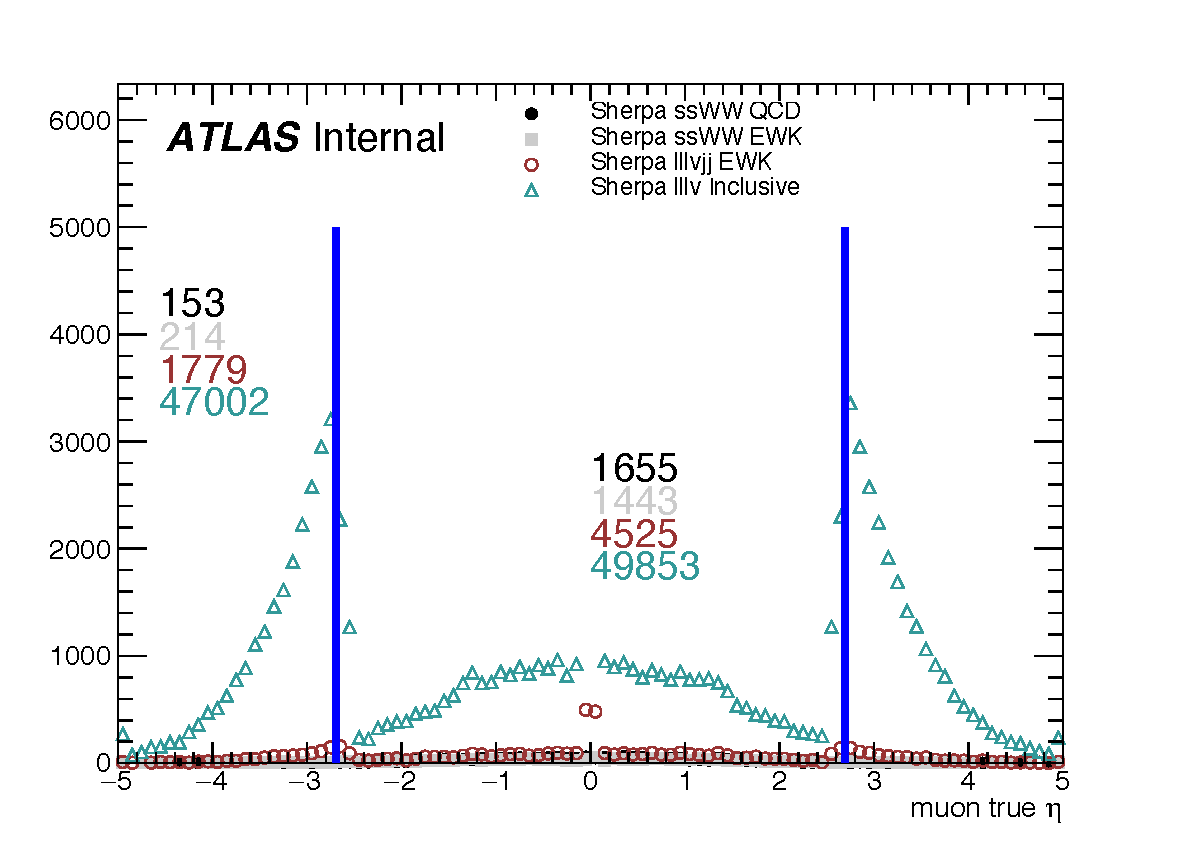
\includegraphics[width=.48\textwidth]{figs/ssww_13tev/custom_or/ExtraMuonEta_counted}
  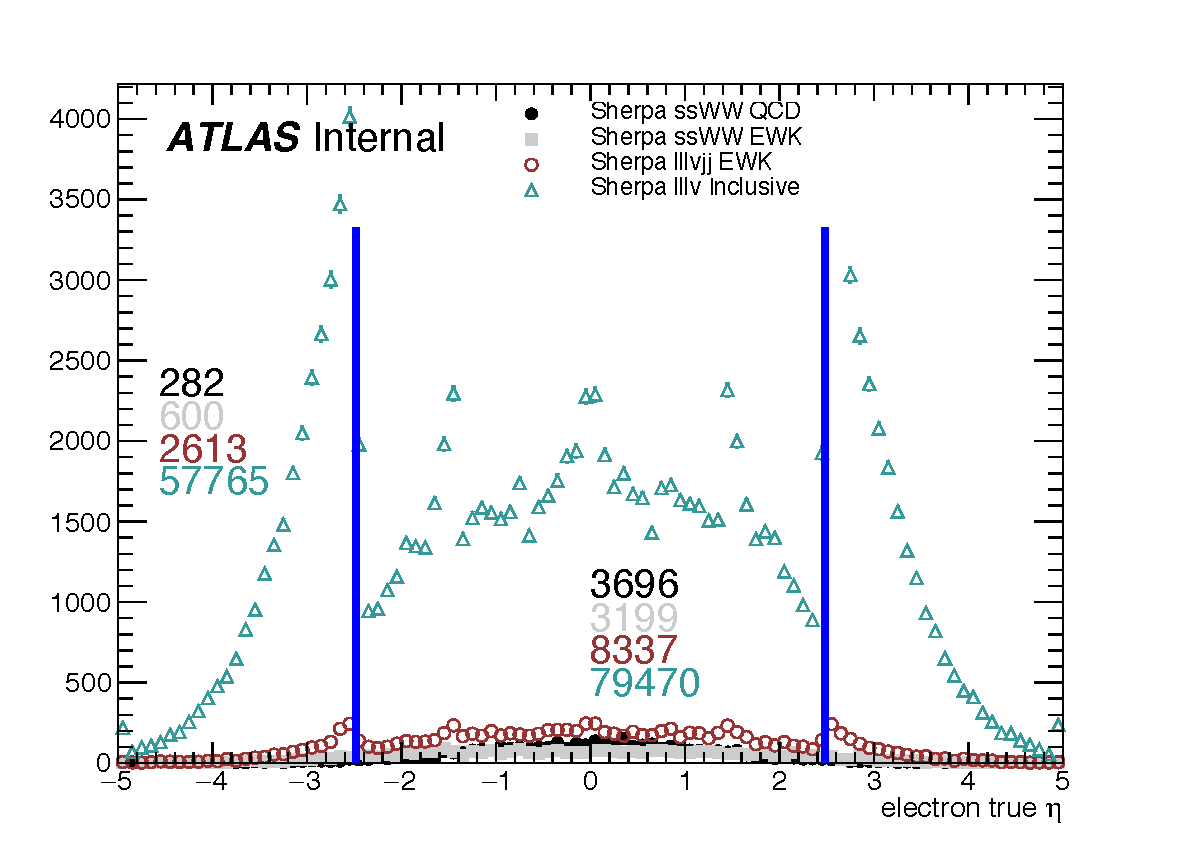
\includegraphics[width=.48\textwidth]{figs/ssww_13tev/custom_or/ExtraElecEta_counted}
  \caption{Pseudorapidity ($\eta$) distributions of truth muons (top) and electrons (bottom) for Sherpa \ssww and $WZ$ MC samples.  The blue vertical lines represent the allowed $\eta$ range for each lepton flavor.  The numbers correspond to the number of raw MC events that fall within and outside of the allowed $\eta$ range for each MC sample.}
  \label{fig:ssww13tev_wzveto_truthlepeta}
\end{figure}

In order to construct this custom OR, a new quantity is defined between a lepton ($l$) and a nearby jet ($j$)
\begin{equation}
  \ptratio(l,j) = \frac{{\pt}_l}{{\pt}_j}%\pt(l)/\pt(j)
  \label{eq:ssww13tev_ptratio}
\end{equation}
which, along with $\deltar(l,j)$, will make up the custom OR criteria.
The idea behind including $\ptratio$ is to be able to preferentially remove background leptons originating from jets (those that carry a low percentage of the total jet momentum) instead of removing \emph{any} lepton near a jet.
The distributions of $\ptratio$ and the associated efficiency curves for muons and electrons can be found in Figures~\ref{fig:ssww13tev_ptratio_muon} and \ref{fig:ssww13tev_ptratio_elec}, respectively, and the distributions for $\deltar(\mu,j)$ for muons can be found in Figure~\ref{fig:ssww13tev_drlj_muon}.
Since all electrons have an associated jet in the calorimeters, the $\deltar(e,j)$ variable is not a good quantity to use for this custom OR.

\begin{figure}[htbp]
  \centering
  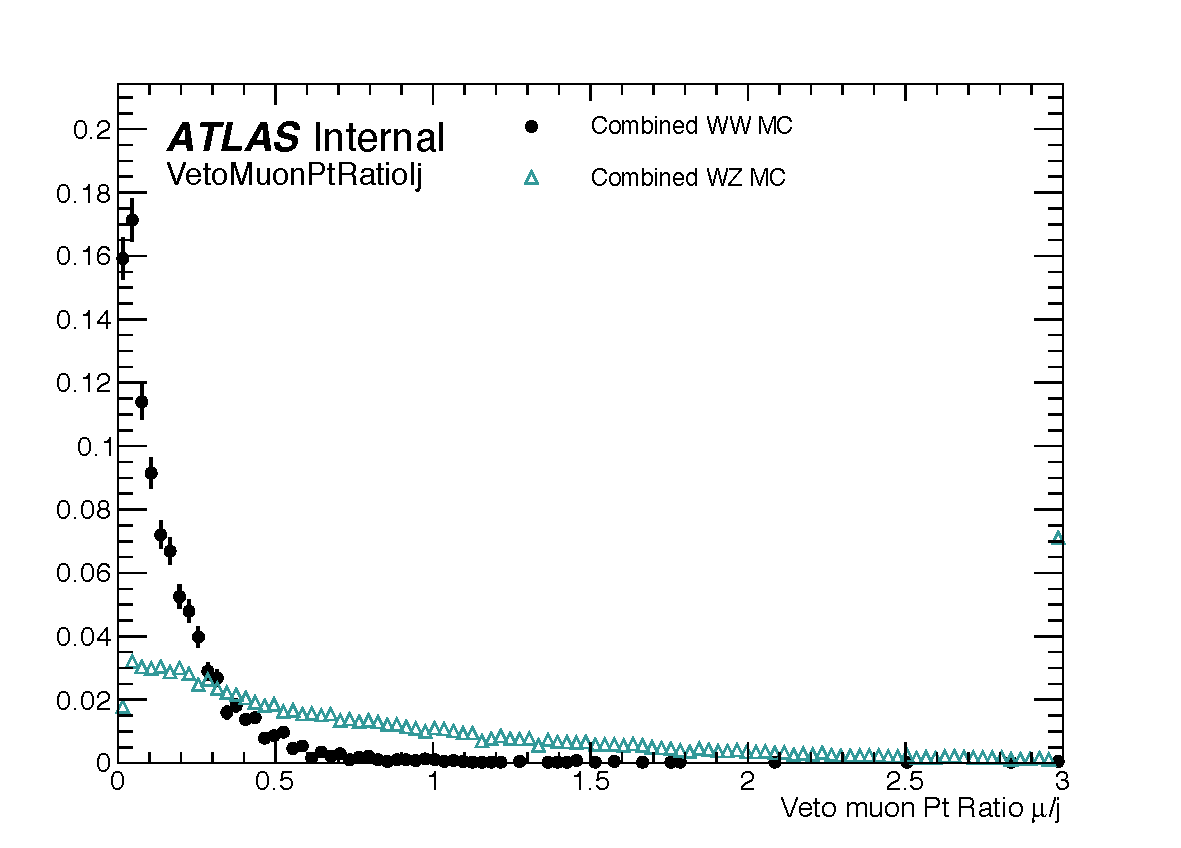
\includegraphics[width=.48\textwidth]{figs/ssww_13tev/custom_or/VetoMuonPtRatiolj}
  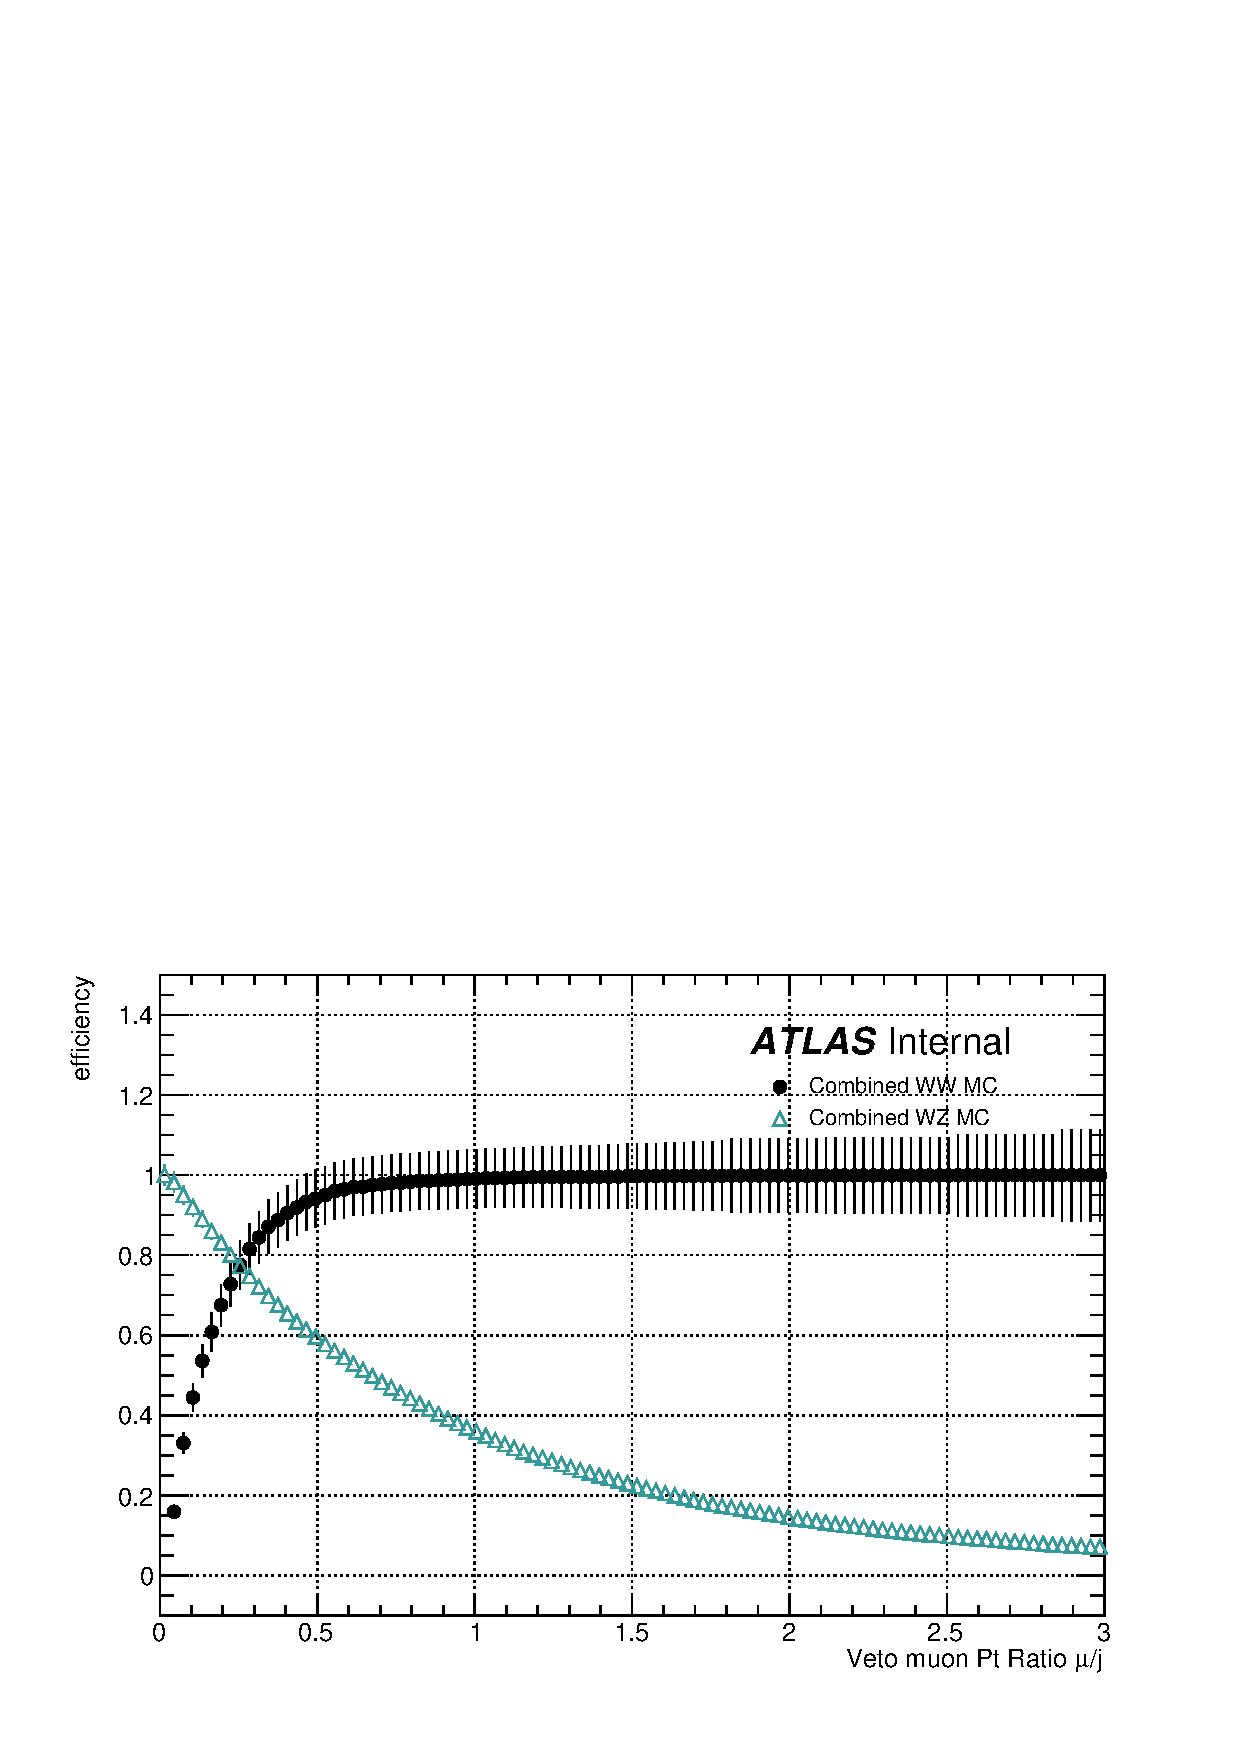
\includegraphics[width=.48\textwidth]{figs/ssww_13tev/custom_or/ROC_VetoMuonPtRatiolj}
  \caption{Distributions of $\ptratio(\mu,j)$ for EWK and QCD \ssww signal (black) and $WZ$ background (teal) for truth-matched third muons in events that pass the trilepton veto.  Both distributions are normalized to unit area.  The associated efficiency curves are on the right where efficiency is defined as the percentage of total events that would pass a cut on $\ptratio(\mu,j)$ at a given value on the $x$-axis.}
  \label{fig:ssww13tev_ptratio_muon}
\end{figure}

\begin{figure}[htbp]
  \centering      
  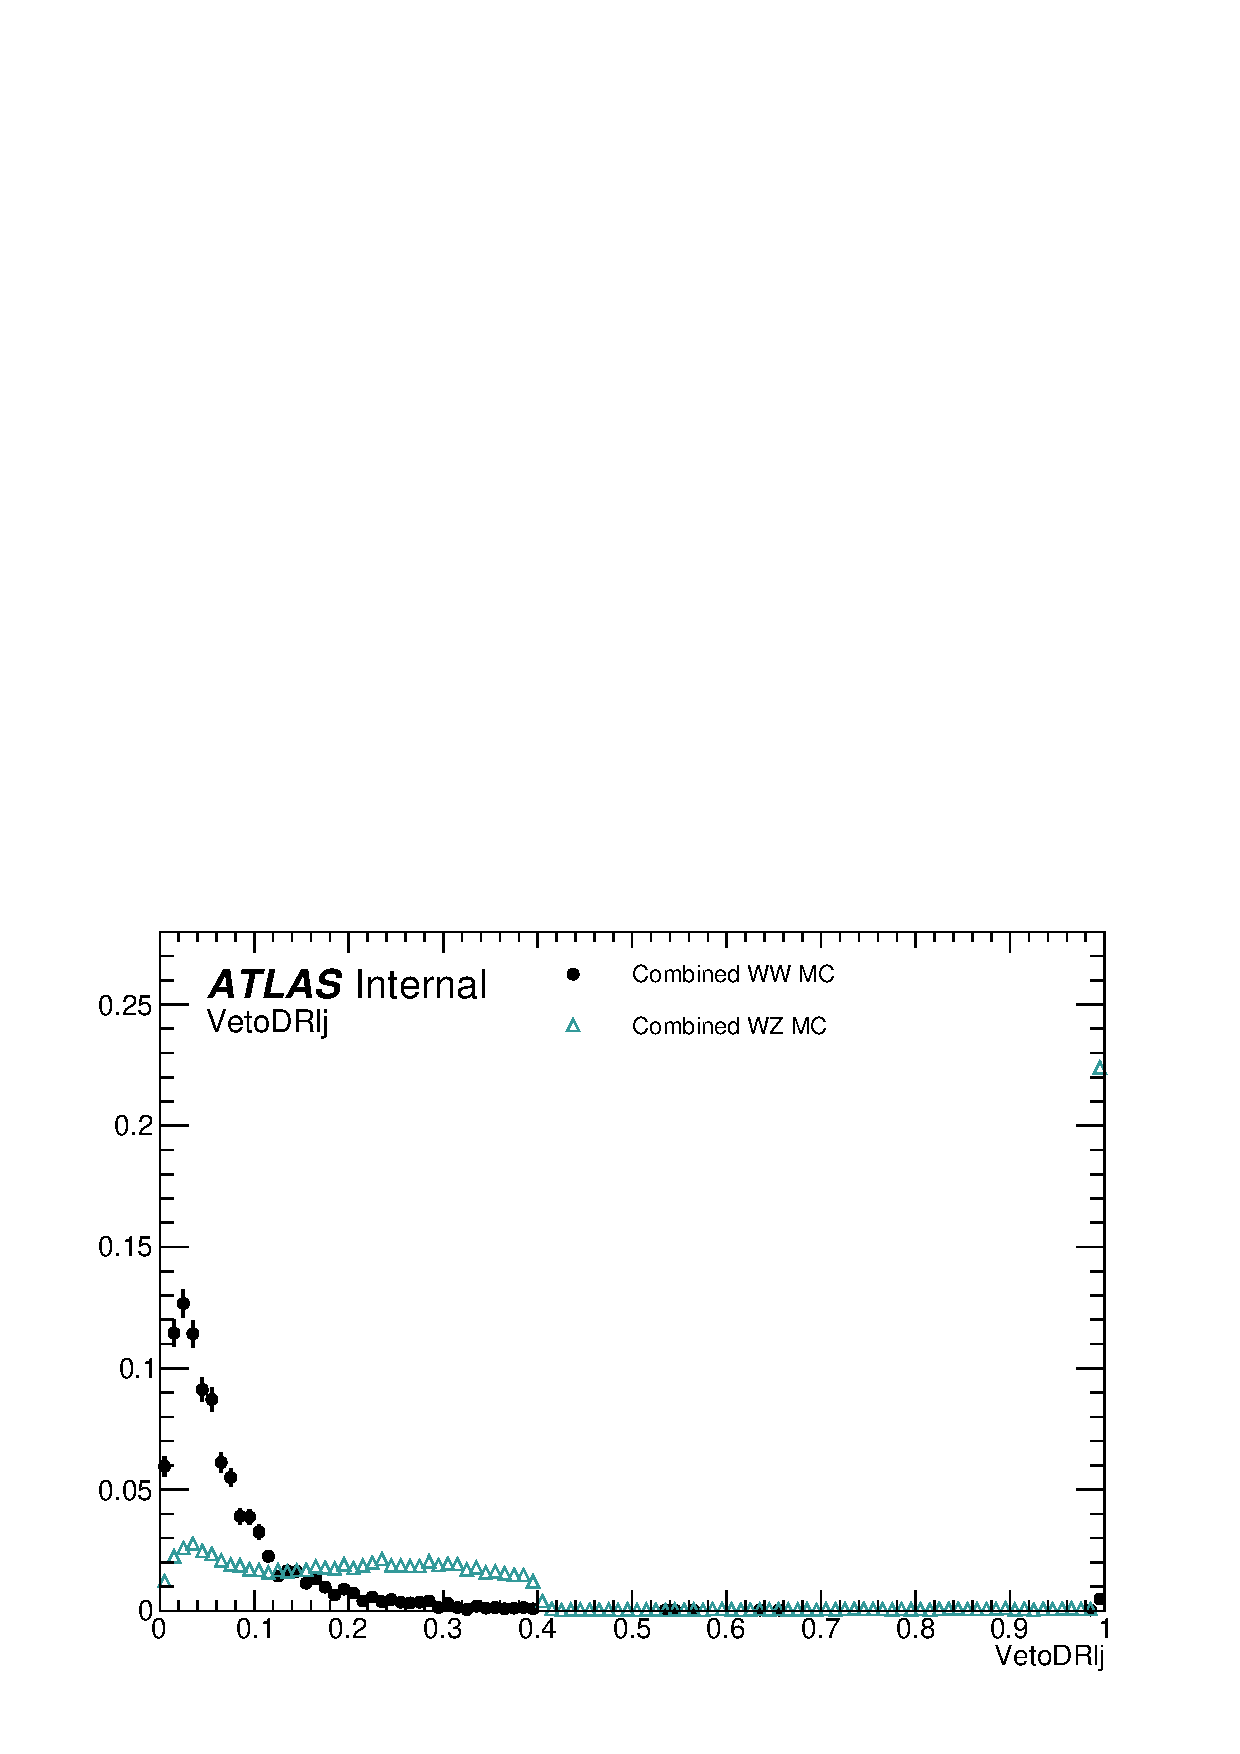
\includegraphics[width=.48\textwidth]{figs/ssww_13tev/custom_or/veto_muon_VetoDRlj}
  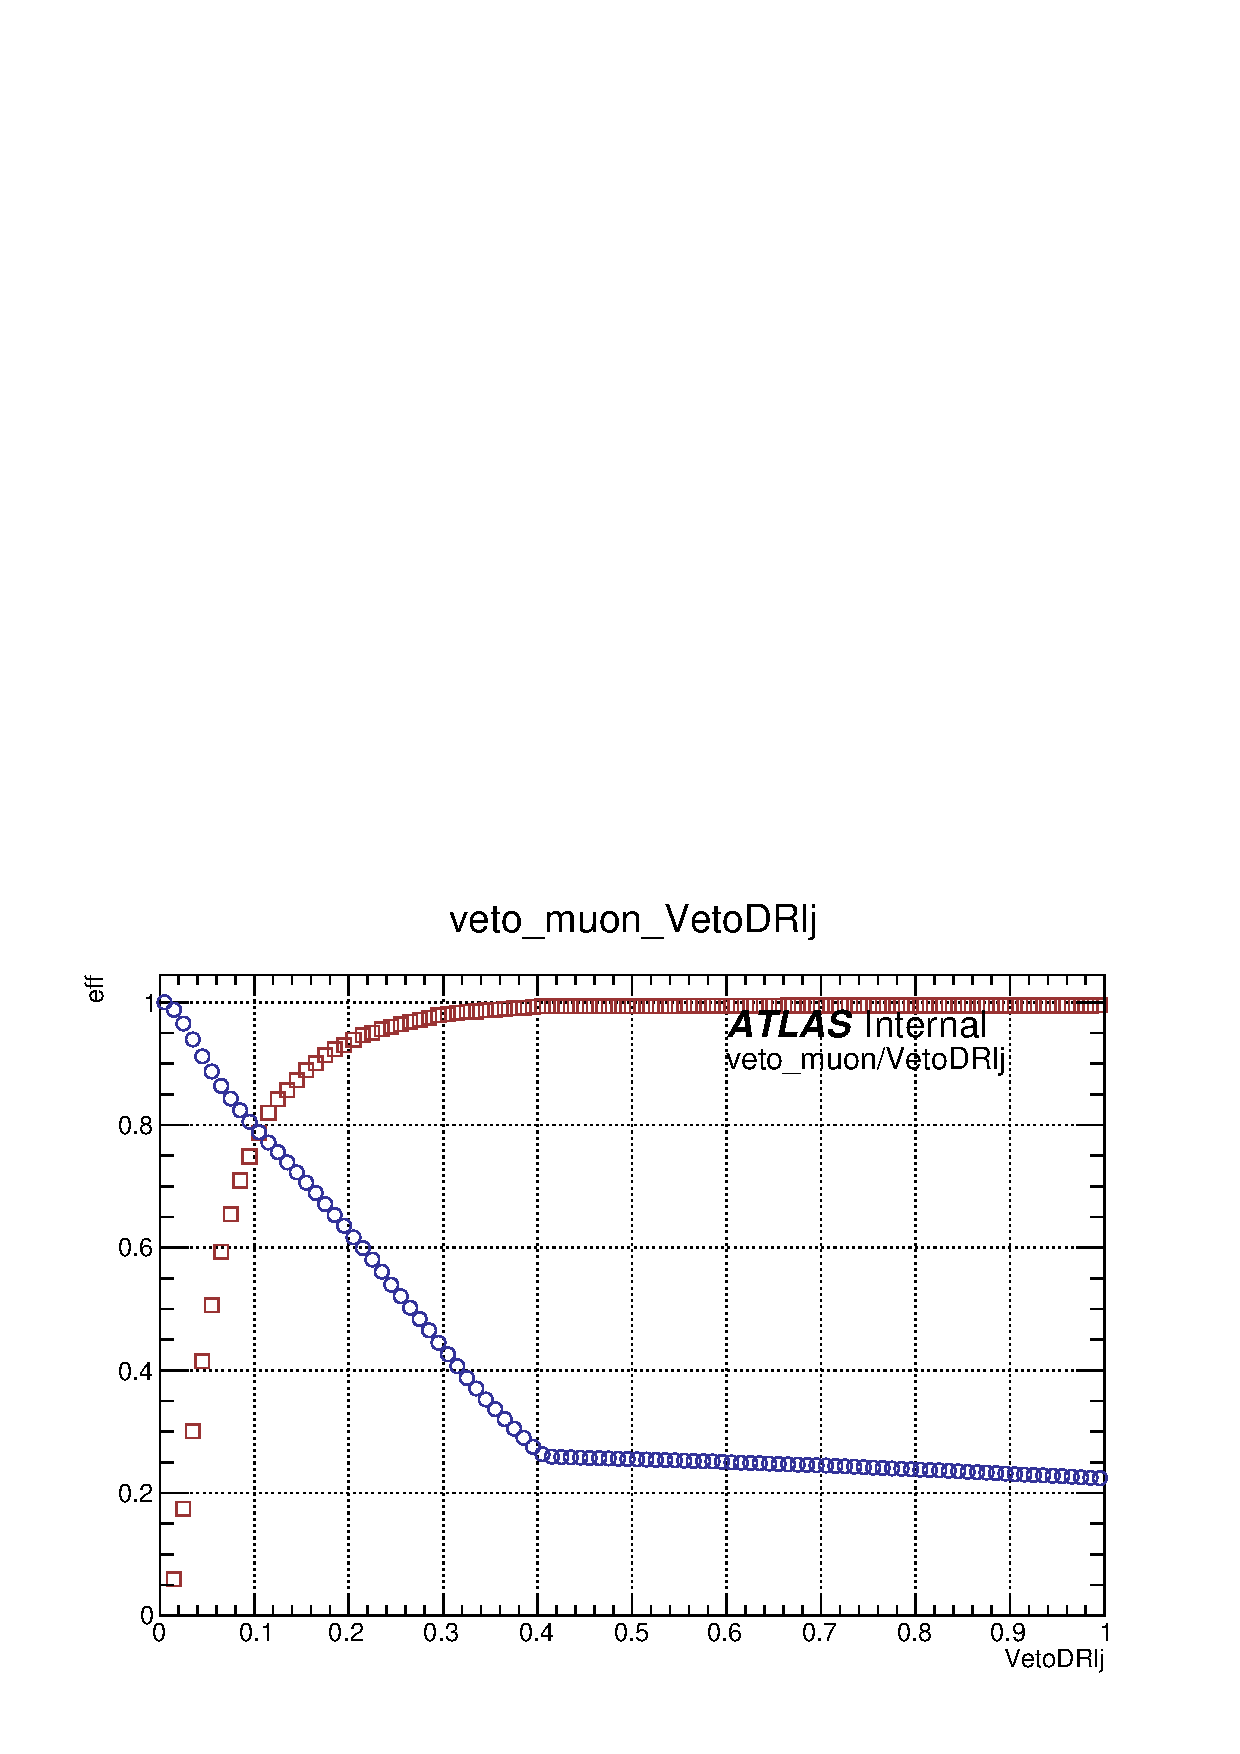
\includegraphics[width=.48\textwidth]{figs/ssww_13tev/custom_or/ROC_veto_muon_VetoDRlj}\\
  \caption{Distributions of $\deltar(\mu,j)$ for EWK and QCD \ssww signal (black) and $WZ$ background (teal) for truth-matched third muons in events that pass the trilepton veto.  Both distributions are normalized to unit area.  The associated efficiency curves are on the right where efficiency is defined as the percentage of total events that would pass a cut on $\deltar(\mu,j)$ at a given value on the $x$-axis.}
  \label{fig:ssww13tev_drlj_muon}
\end{figure}

\begin{figure}[htbp]
  \centering
  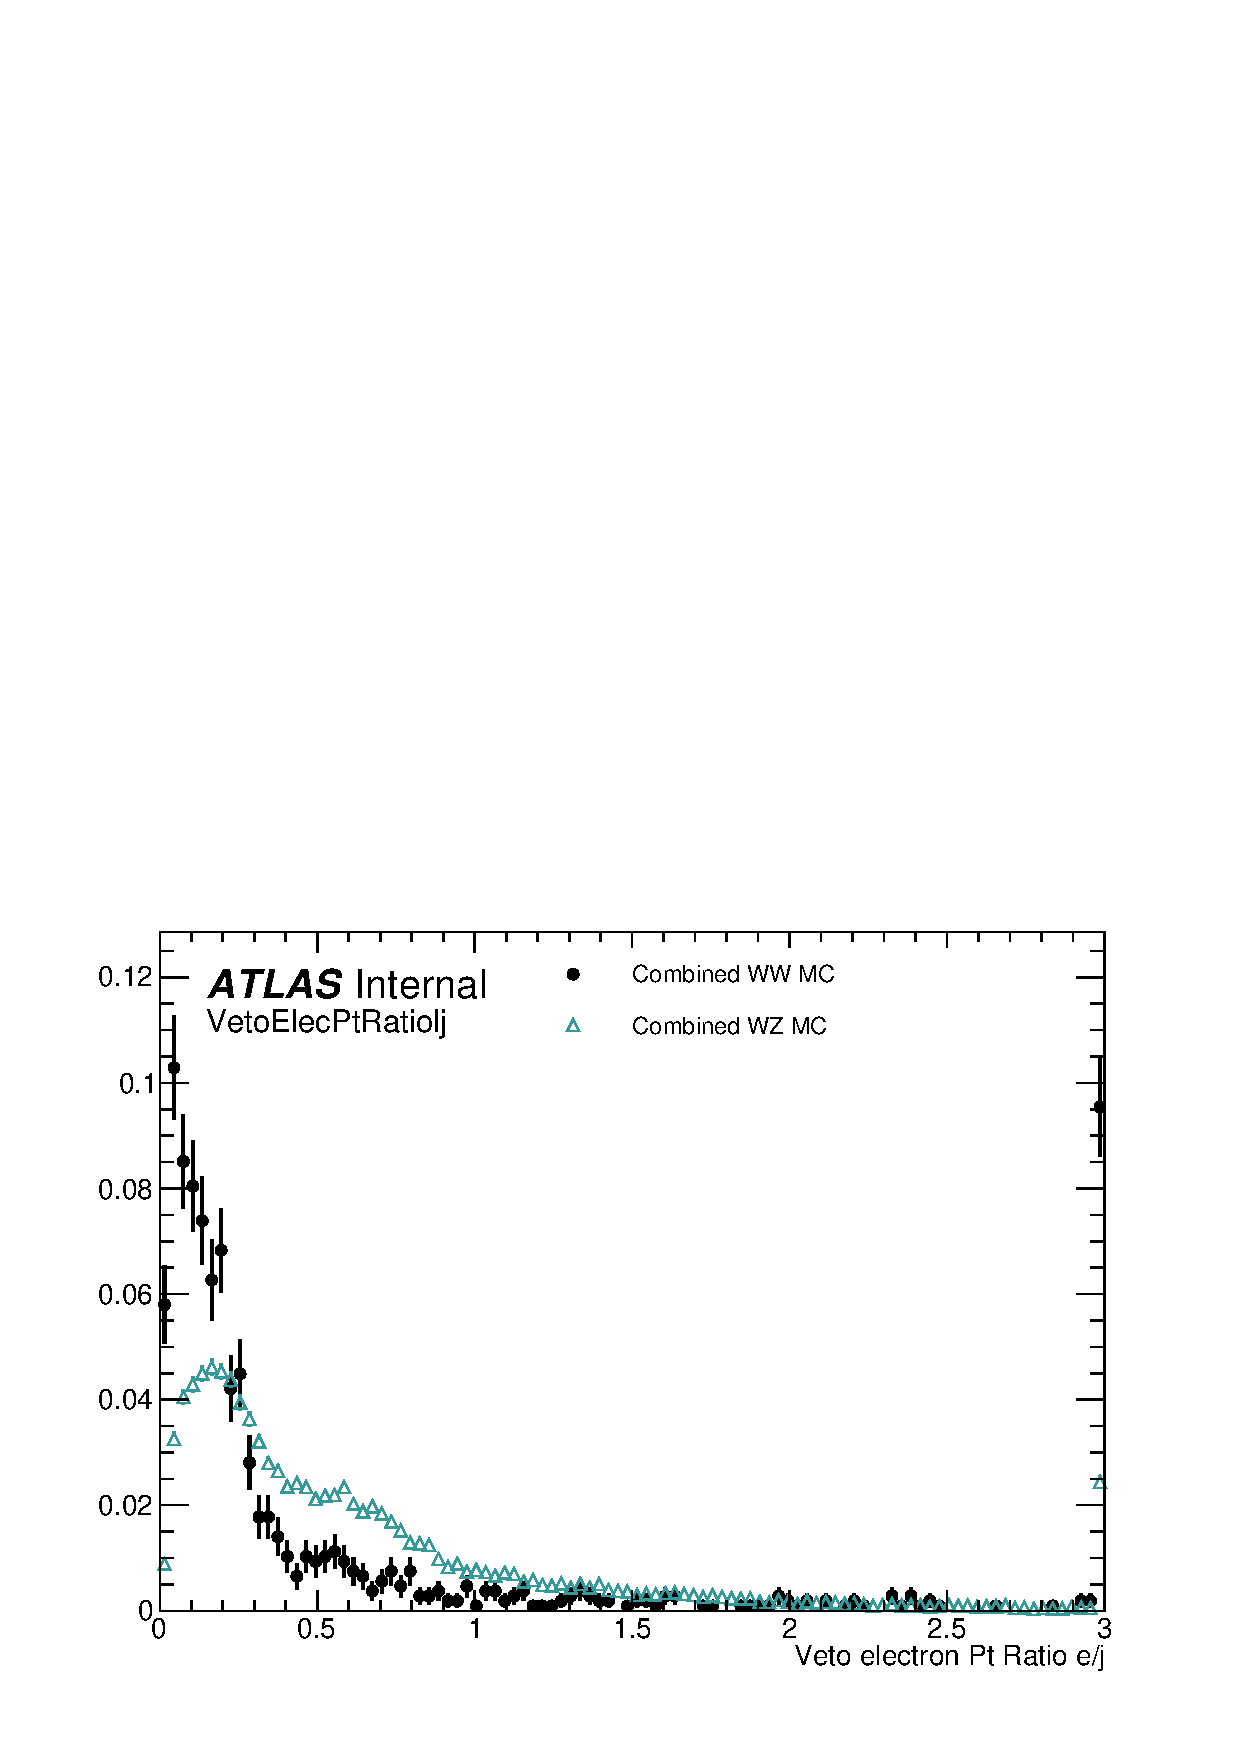
\includegraphics[width=.48\textwidth]{figs/ssww_13tev/custom_or/VetoElecPtRatiolj}
  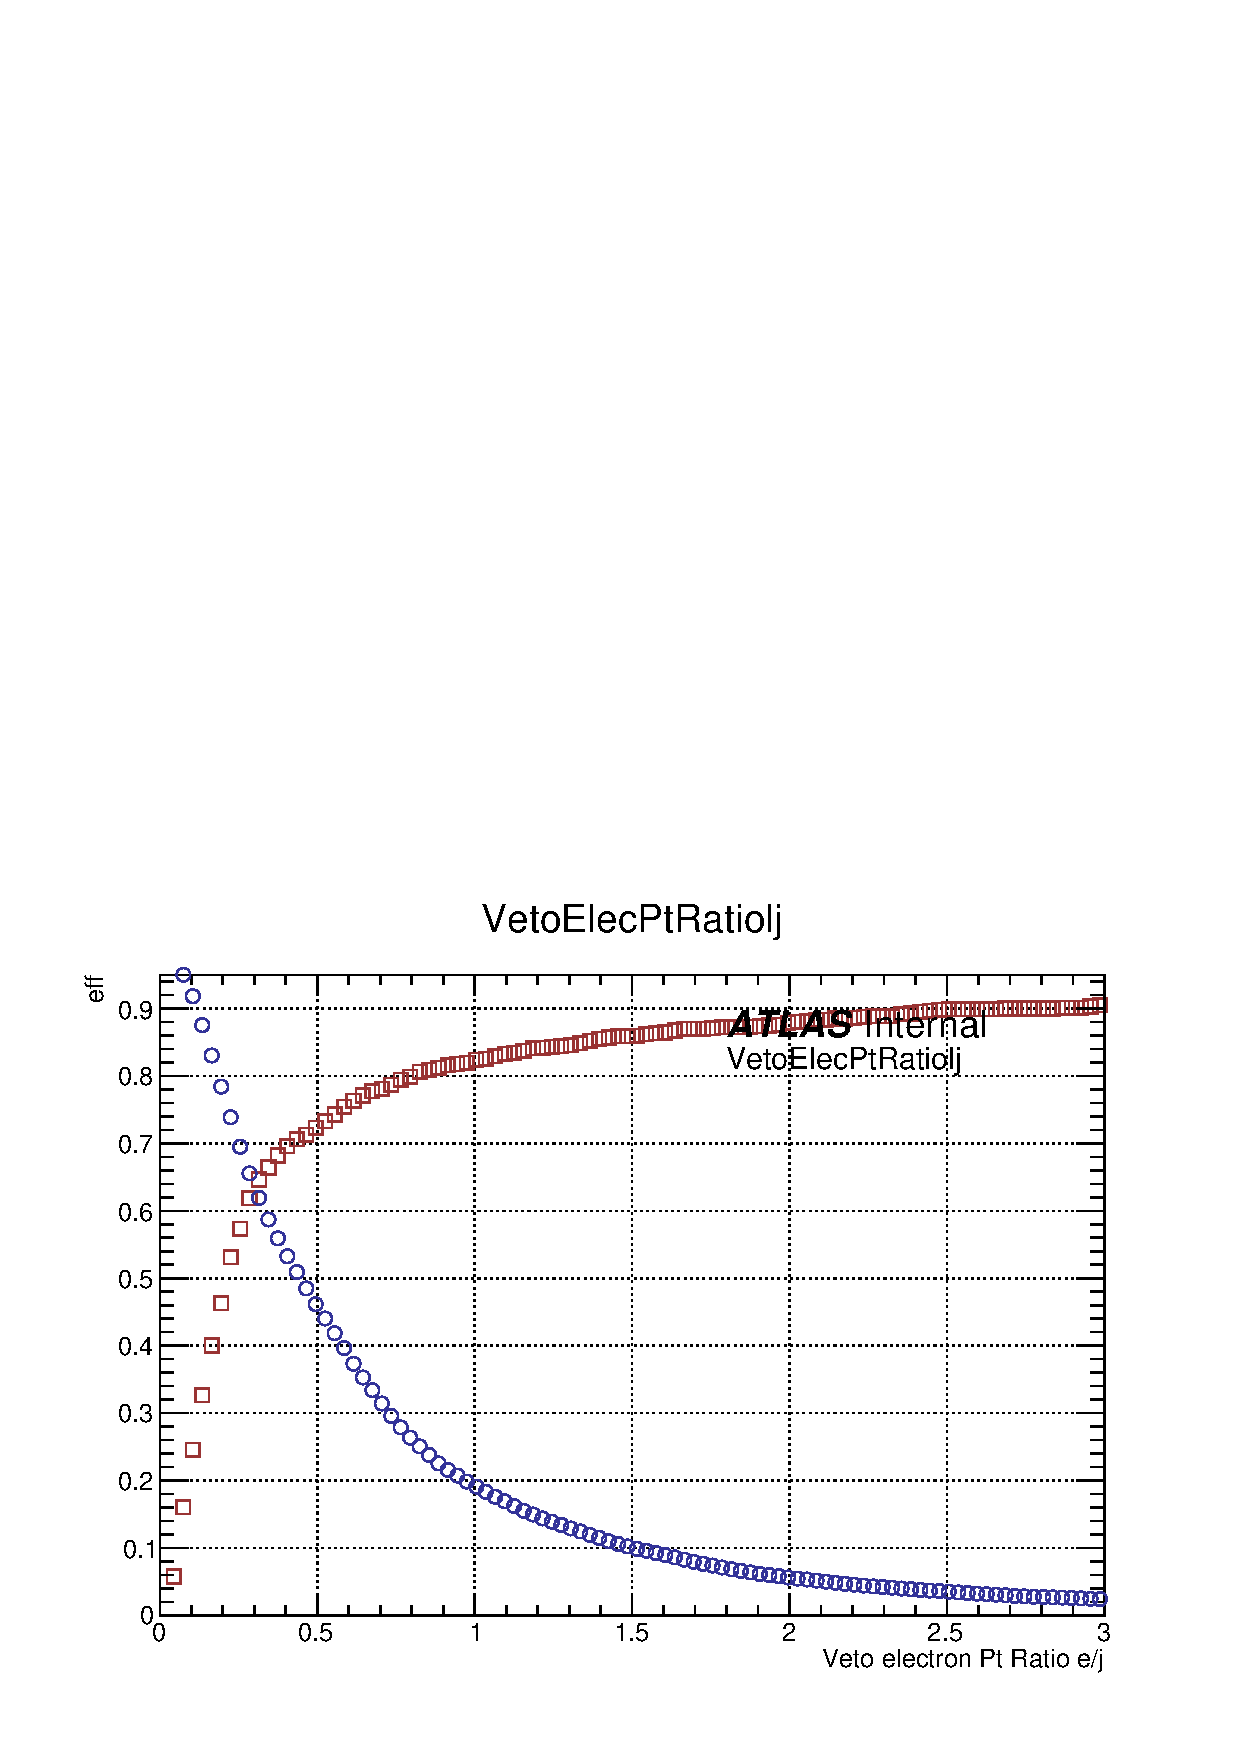
\includegraphics[width=.48\textwidth]{figs/ssww_13tev/custom_or/ROC_VetoElecPtRatiolj}
  \caption{Distributions of $\ptratio(e,j)$ for EWK and QCD \ssww signal (black) and $WZ$ background (teal) for truth-matched third electrons in events that pass the trilepton veto.  Both distributions are normalized to unit area.  The associated efficiency curves are on the right where efficiency is defined as the percentage of total events that would pass a cut on $\ptratio(e,j)$ at a given value on the $x$-axis.}
  \label{fig:ssww13tev_ptratio_elec}
\end{figure}

A working point for the Custom OR was chosen by requiring 90\% signal retention for muons and 90\% background rejection for electrons.
The cut on electrons was allowed to be much tighter because the number of signal events with a third electron is considerably smaller than for muons.
It should be emphasized that the signal events present in Figures~\ref{fig:ssww13tev_ptratio_muon}-\ref{fig:ssww13tev_ptratio_elec} do not represent the full set of signal events, but only those with a real third lepton (which must come from some source other than the signal \ssww process).
For muons, a logical `or' of $\ptratio(\mu,j)$ and $\deltar(\mu,j)$ is used to maximize the third lepton acceptance due to correlations between the quantities, as shown in Figure~\ref{fig:ssww13tev_customor_muon_2d}; for electrons, only a cut on $\ptratio(e,j)$ is used.
The Custom OR working point is defined in Table~\ref{tab:custom_or_definition}.

\begin{table}[htbp]
  \centering
  \begin{tabular}{l | c}
    \multicolumn{2}{c}{Custom OR Definition} \\
    \hline\hline
    Muons     & $\ptratio(\mu,j) > 0.40$ or $\deltar(\mu,j) > 0.15$\\
    Electrons & $\ptratio(e,j) > 0.18$ \\
    \hline
  \end{tabular}
  \caption{Custom OR definition.  Leptons must pass this selection in order to be counted for the trilepton veto.}
  \label{tab:custom_or_definition}
\end{table}

\begin{figure}[htbp]
  \centering
  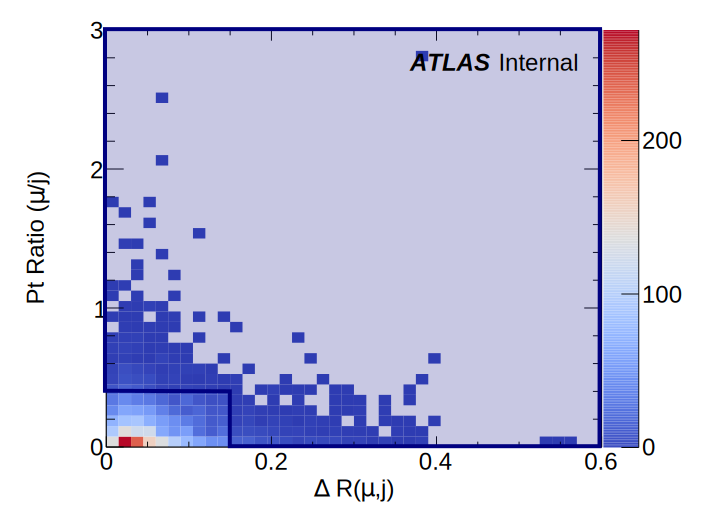
\includegraphics[width=.48\textwidth]{figs/ssww_13tev/custom_or/sig_Muon_DR_PtRatio_edited}
  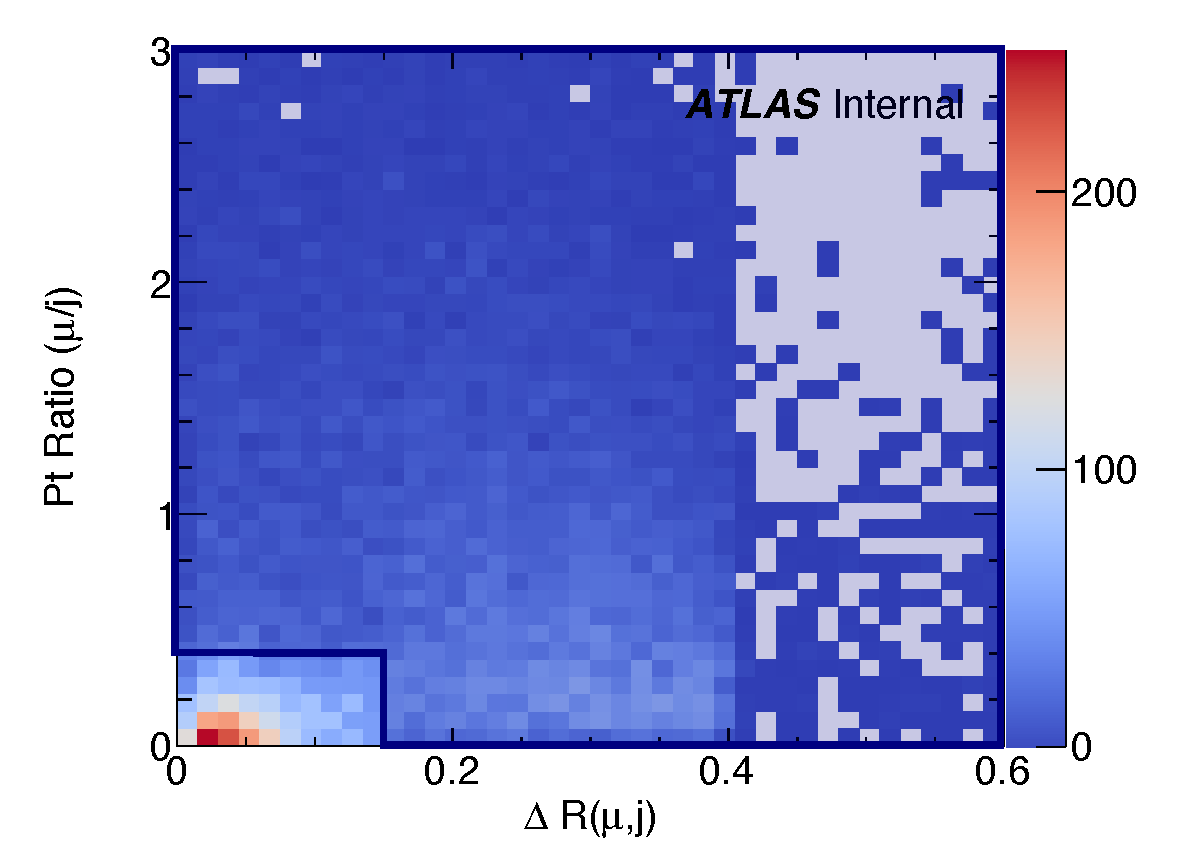
\includegraphics[width=.48\textwidth]{figs/ssww_13tev/custom_or/bkg_Muon_DR_PtRatio_edited}
  \caption{Two-dimensional plots of $\ptratio(\mu,j)$ vs $\deltar(\mu,j)$ for truth-matched third muons in events that pass the trilepton veto for EWK and QCD \ssww signal (left) and $WZ$ background (right).  The blue overlay indicates the area in which the third leptons will pass the custom OR and result in the event failing the trilepton veto.}
  \label{fig:ssww13tev_customor_muon_2d}
\end{figure}

Initial tests of the performance of the Custom OR yielded promising results, with approximately 20\% reduction in $WZ$ background compared to less than 2\% signal loss in the signal region.
Unfortunately, due to differences between the primary analysis framework and the one used for testing, in practice the gains in $WZ$ rejection were not nearly as substantial, and ultimately the Custom OR was not included in the final analysis.
However, it is still a potentially useful tool for improving background rejection based on lepton counting in analyses with overly aggressive OR procedures.
